\documentclass[1p]{elsarticle_modified}
%\bibliographystyle{elsarticle-num}

%\usepackage[colorlinks]{hyperref}
%\usepackage{abbrmath_seonhwa} %\Abb, \Ascr, \Acal ,\Abf, \Afrak
\usepackage{amsfonts}
\usepackage{amssymb}
\usepackage{amsmath}
\usepackage{amsthm}
\usepackage{scalefnt}
\usepackage{amsbsy}
\usepackage{kotex}
\usepackage{caption}
\usepackage{subfig}
\usepackage{color}
\usepackage{graphicx}
\usepackage{xcolor} %% white, black, red, green, blue, cyan, magenta, yellow
\usepackage{float}
\usepackage{setspace}
\usepackage{hyperref}

\usepackage{tikz}
\usetikzlibrary{arrows}

\usepackage{multirow}
\usepackage{array} % fixed length table
\usepackage{hhline}

%%%%%%%%%%%%%%%%%%%%%
\makeatletter
\renewcommand*\env@matrix[1][\arraystretch]{%
	\edef\arraystretch{#1}%
	\hskip -\arraycolsep
	\let\@ifnextchar\new@ifnextchar
	\array{*\c@MaxMatrixCols c}}
\makeatother %https://tex.stackexchange.com/questions/14071/how-can-i-increase-the-line-spacing-in-a-matrix
%%%%%%%%%%%%%%%

\usepackage[normalem]{ulem}

\newcommand{\msout}[1]{\ifmmode\text{\sout{\ensuremath{#1}}}\else\sout{#1}\fi}
%SOURCE: \msout is \stkout macro in https://tex.stackexchange.com/questions/20609/strikeout-in-math-mode

\newcommand{\cancel}[1]{
	\ifmmode
	{\color{red}\msout{#1}}
	\else
	{\color{red}\sout{#1}}
	\fi
}

\newcommand{\add}[1]{
	{\color{blue}\uwave{#1}}
}

\newcommand{\replace}[2]{
	\ifmmode
	{\color{red}\msout{#1}}{\color{blue}\uwave{#2}}
	\else
	{\color{red}\sout{#1}}{\color{blue}\uwave{#2}}
	\fi
}

\newcommand{\Sol}{\mathcal{S}} %segment
\newcommand{\D}{D} %diagram
\newcommand{\A}{\mathcal{A}} %arc


%%%%%%%%%%%%%%%%%%%%%%%%%%%%%5 test

\def\sl{\operatorname{\textup{SL}}(2,\Cbb)}
\def\psl{\operatorname{\textup{PSL}}(2,\Cbb)}
\def\quan{\mkern 1mu \triangleright \mkern 1mu}

\theoremstyle{definition}
\newtheorem{thm}{Theorem}[section]
\newtheorem{prop}[thm]{Proposition}
\newtheorem{lem}[thm]{Lemma}
\newtheorem{ques}[thm]{Question}
\newtheorem{cor}[thm]{Corollary}
\newtheorem{defn}[thm]{Definition}
\newtheorem{exam}[thm]{Example}
\newtheorem{rmk}[thm]{Remark}
\newtheorem{alg}[thm]{Algorithm}

\newcommand{\I}{\sqrt{-1}}
\begin{document}

%\begin{frontmatter}
%
%\title{Boundary parabolic representations of knots up to 8 crossings}
%
%%% Group authors per affiliation:
%\author{Yunhi Cho} 
%\address{Department of Mathematics, University of Seoul, Seoul, Korea}
%\ead{yhcho@uos.ac.kr}
%
%
%\author{Seonhwa Kim} %\fnref{s_kim}}
%\address{Center for Geometry and Physics, Institute for Basic Science, Pohang, 37673, Korea}
%\ead{ryeona17@ibs.re.kr}
%
%\author{Hyuk Kim}
%\address{Department of Mathematical Sciences, Seoul National University, Seoul 08826, Korea}
%\ead{hyukkim@snu.ac.kr}
%
%\author{Seokbeom Yoon}
%\address{Department of Mathematical Sciences, Seoul National University, Seoul, 08826,  Korea}
%\ead{sbyoon15@snu.ac.kr}
%
%\begin{abstract}
%We find all boundary parabolic representation of knots up to 8 crossings.
%
%\end{abstract}
%\begin{keyword}
%    \MSC[2010] 57M25 
%\end{keyword}
%
%\end{frontmatter}

%\linenumbers
%\tableofcontents
%
\newcommand\colored[1]{\textcolor{white}{\rule[-0.35ex]{0.8em}{1.4ex}}\kern-0.8em\color{red} #1}%
%\newcommand\colored[1]{\textcolor{white}{ #1}\kern-2.17ex	\textcolor{white}{ #1}\kern-1.81ex	\textcolor{white}{ #1}\kern-2.15ex\color{red}#1	}

{\Large $\underline{11a_{148}~(K11a_{148})}$}

\setlength{\tabcolsep}{10pt}
\renewcommand{\arraystretch}{1.6}
\vspace{1cm}\begin{tabular}{m{100pt}>{\centering\arraybackslash}m{274pt}}
\multirow{5}{120pt}{
	\centering
	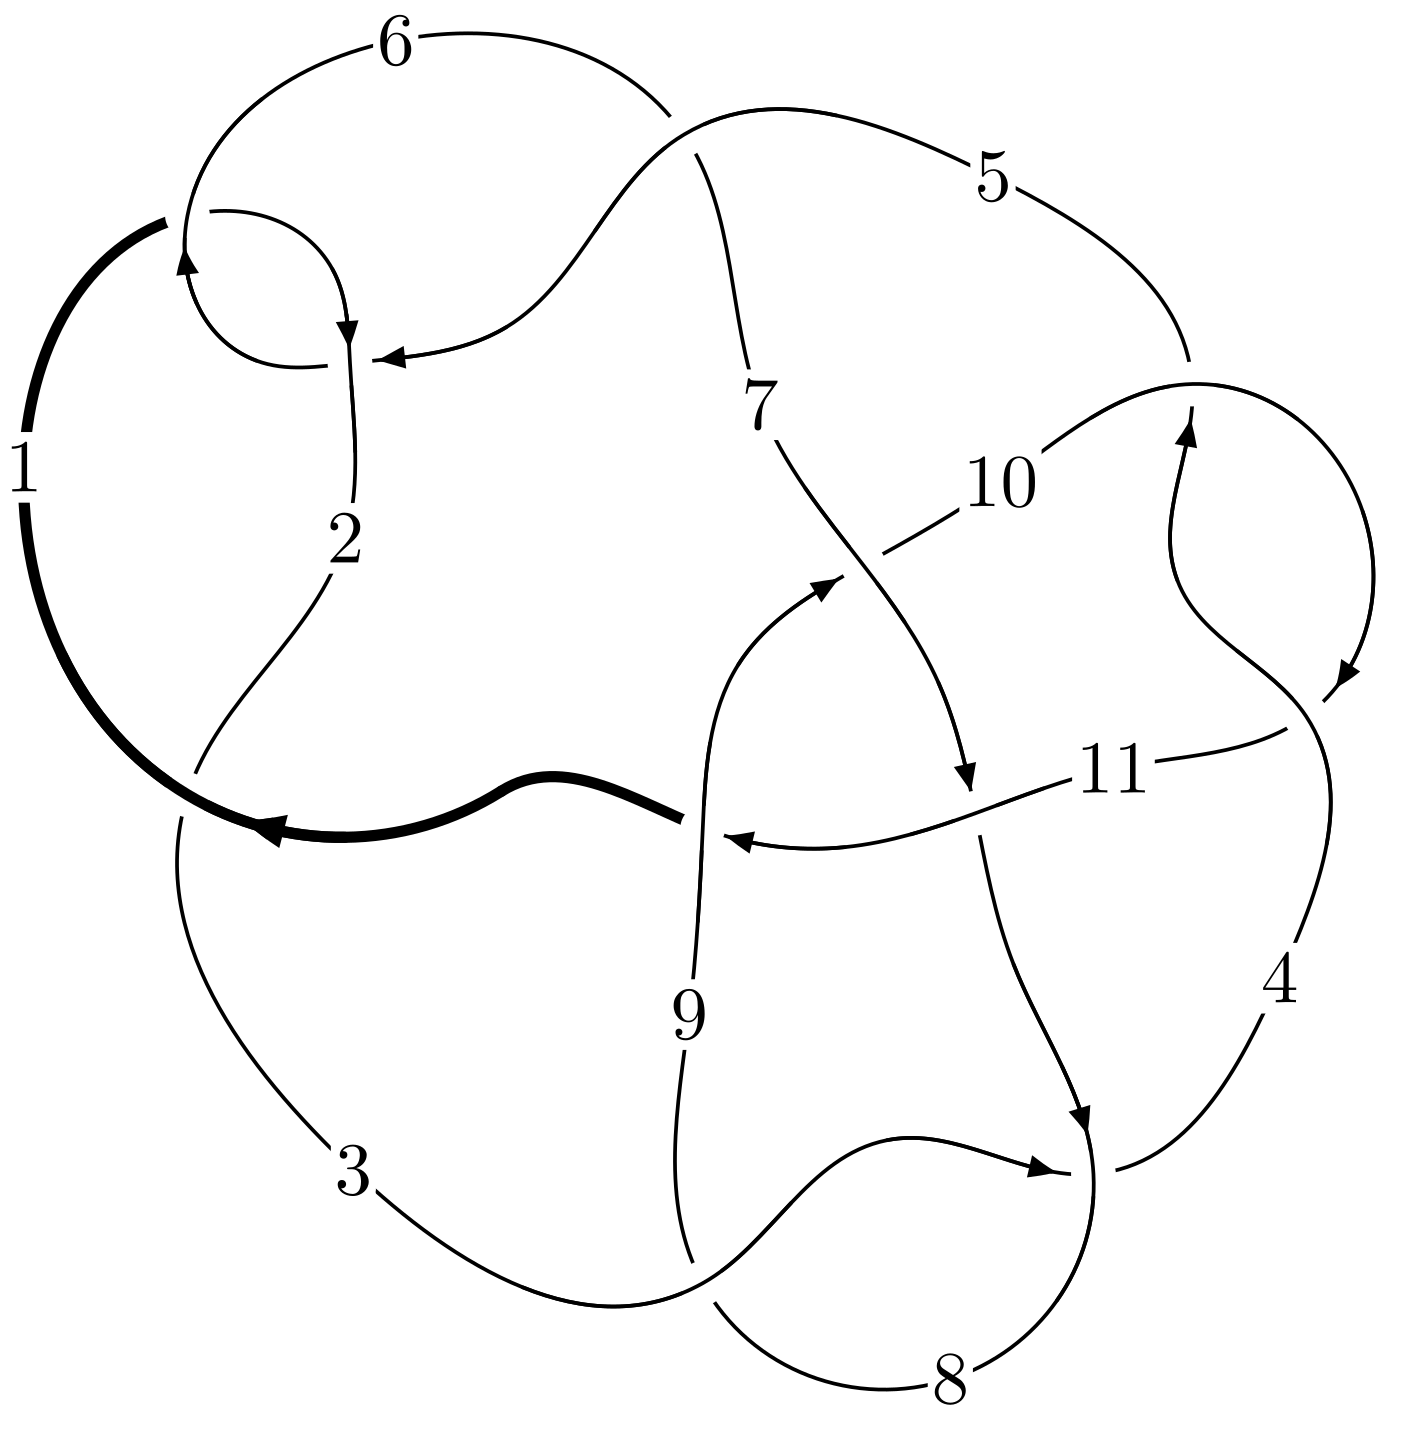
\includegraphics[width=112pt]{../../../GIT/diagram.site/Diagrams/png/397_11a_148.png}\\
\ \ \ A knot diagram\footnotemark}&
\allowdisplaybreaks
\textbf{Linearized knot diagam} \\
\cline{2-2}
 &
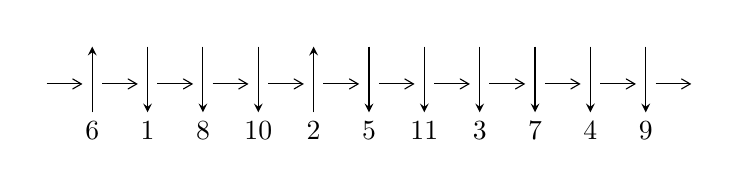
\begin{tikzpicture}[x=20pt, y=17pt]
	% nodes
	\node (C0) at (0, 0) {};
	\node (C1) at (1, 0) {};
	\node (C1U) at (1, +1) {};
	\node (C1D) at (1, -1) {6};

	\node (C2) at (2, 0) {};
	\node (C2U) at (2, +1) {};
	\node (C2D) at (2, -1) {1};

	\node (C3) at (3, 0) {};
	\node (C3U) at (3, +1) {};
	\node (C3D) at (3, -1) {8};

	\node (C4) at (4, 0) {};
	\node (C4U) at (4, +1) {};
	\node (C4D) at (4, -1) {10};

	\node (C5) at (5, 0) {};
	\node (C5U) at (5, +1) {};
	\node (C5D) at (5, -1) {2};

	\node (C6) at (6, 0) {};
	\node (C6U) at (6, +1) {};
	\node (C6D) at (6, -1) {5};

	\node (C7) at (7, 0) {};
	\node (C7U) at (7, +1) {};
	\node (C7D) at (7, -1) {11};

	\node (C8) at (8, 0) {};
	\node (C8U) at (8, +1) {};
	\node (C8D) at (8, -1) {3};

	\node (C9) at (9, 0) {};
	\node (C9U) at (9, +1) {};
	\node (C9D) at (9, -1) {7};

	\node (C10) at (10, 0) {};
	\node (C10U) at (10, +1) {};
	\node (C10D) at (10, -1) {4};

	\node (C11) at (11, 0) {};
	\node (C11U) at (11, +1) {};
	\node (C11D) at (11, -1) {9};
	\node (C12) at (12, 0) {};

	% arrows
	\draw[->,>={angle 60}]
	(C0) edge (C1) (C1) edge (C2) (C2) edge (C3) (C3) edge (C4) (C4) edge (C5) (C5) edge (C6) (C6) edge (C7) (C7) edge (C8) (C8) edge (C9) (C9) edge (C10) (C10) edge (C11) (C11) edge (C12) ;	\draw[->,>=stealth]
	(C1D) edge (C1U) (C2U) edge (C2D) (C3U) edge (C3D) (C4U) edge (C4D) (C5D) edge (C5U) (C6U) edge (C6D) (C7U) edge (C7D) (C8U) edge (C8D) (C9U) edge (C9D) (C10U) edge (C10D) (C11U) edge (C11D) ;
	\end{tikzpicture} \\
\hhline{~~} \\& 
\textbf{Solving Sequence} \\ \cline{2-2} 
 &
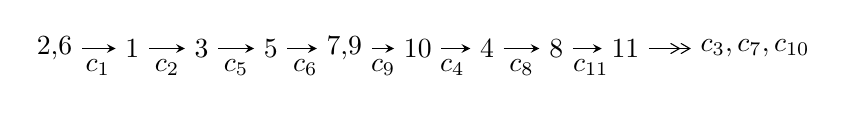
\begin{tikzpicture}[x=25pt, y=7pt]
	% node
	\node (A0) at (-1/8, 0) {2,6};
	\node (A1) at (1, 0) {1};
	\node (A2) at (2, 0) {3};
	\node (A3) at (3, 0) {5};
	\node (A4) at (65/16, 0) {7,9};
	\node (A5) at (41/8, 0) {10};
	\node (A6) at (49/8, 0) {4};
	\node (A7) at (57/8, 0) {8};
	\node (A8) at (65/8, 0) {11};
	\node (C1) at (1/2, -1) {$c_{1}$};
	\node (C2) at (3/2, -1) {$c_{2}$};
	\node (C3) at (5/2, -1) {$c_{5}$};
	\node (C4) at (7/2, -1) {$c_{6}$};
	\node (C5) at (37/8, -1) {$c_{9}$};
	\node (C6) at (45/8, -1) {$c_{4}$};
	\node (C7) at (53/8, -1) {$c_{8}$};
	\node (C8) at (61/8, -1) {$c_{11}$};
	\node (A9) at (10, 0) {$c_{3},c_{7},c_{10}$};

	% edge
	\draw[->,>=stealth]	
	(A0) edge (A1) (A1) edge (A2) (A2) edge (A3) (A3) edge (A4) (A4) edge (A5) (A5) edge (A6) (A6) edge (A7) (A7) edge (A8) ;
	\draw[->>,>={angle 60}]	
	(A8) edge (A9);
\end{tikzpicture} \\ 

\end{tabular} \\

\footnotetext{
The image of knot diagram is generated by the software ``\textbf{Draw programme}" developed by Andrew Bartholomew(\url{http://www.layer8.co.uk/maths/draw/index.htm\#Running-draw}), where we modified some parts for our purpose(\url{https://github.com/CATsTAILs/LinksPainter}).
}\phantom \\ \newline 
\centering \textbf{Ideals for irreducible components\footnotemark of $X_{\text{par}}$} 
 
\begin{align*}
I^u_{1}&=\langle 
35 u^{24}+168 u^{23}+\cdots+2 b-32,\;-27 u^{24}-155 u^{23}+\cdots+2 a+101,\;u^{25}+6 u^{24}+\cdots+2 u-4\rangle \\
I^u_{2}&=\langle 
2016599941 u^{10} a^3-15792956111 u^{10} a^2+\cdots+42968527616 a+47798397673,\\
\phantom{I^u_{2}}&\phantom{= \langle  }2 u^{10} a^3+5 u^{10} a^2+\cdots-11 a-4,\;u^{11}- u^{10}+2 u^9- u^8+4 u^7-2 u^6+4 u^5- u^4+3 u^3+u^2+1\rangle \\
I^u_{3}&=\langle 
- u^{11}+u^{10}-3 u^9+u^8-6 u^7+2 u^6-9 u^5+2 u^4-7 u^3+b-4 u,\\
\phantom{I^u_{3}}&\phantom{= \langle  }u^{11}-2 u^{10}+4 u^9-4 u^8+7 u^7-8 u^6+11 u^5-11 u^4+9 u^3-7 u^2+a+4 u-4,\\
\phantom{I^u_{3}}&\phantom{= \langle  }u^{12}- u^{11}+3 u^{10}-2 u^9+6 u^8-4 u^7+9 u^6-5 u^5+8 u^4-3 u^3+5 u^2- u+1\rangle \\
\\
\end{align*}
\raggedright * 3 irreducible components of $\dim_{\mathbb{C}}=0$, with total 81 representations.\\
\footnotetext{All coefficients of polynomials are rational numbers. But the coefficients are sometimes approximated in decimal forms when there is not enough margin.}
\newpage
\renewcommand{\arraystretch}{1}
\centering \section*{I. $I^u_{1}= \langle 35 u^{24}+168 u^{23}+\cdots+2 b-32,\;-27 u^{24}-155 u^{23}+\cdots+2 a+101,\;u^{25}+6 u^{24}+\cdots+2 u-4 \rangle$}
\flushleft \textbf{(i) Arc colorings}\\
\begin{tabular}{m{7pt} m{180pt} m{7pt} m{180pt} }
\flushright $a_{2}=$&$\begin{pmatrix}1\\0\end{pmatrix}$ \\
\flushright $a_{6}=$&$\begin{pmatrix}0\\u\end{pmatrix}$ \\
\flushright $a_{1}=$&$\begin{pmatrix}1\\u^2\end{pmatrix}$ \\
\flushright $a_{3}=$&$\begin{pmatrix}u^2+1\\u^4\end{pmatrix}$ \\
\flushright $a_{5}=$&$\begin{pmatrix}- u\\u\end{pmatrix}$ \\
\flushright $a_{7}=$&$\begin{pmatrix}- u^3\\u^3+u\end{pmatrix}$ \\
\flushright $a_{9}=$&$\begin{pmatrix}\frac{27}{2} u^{24}+\frac{155}{2} u^{23}+\cdots+39 u-\frac{101}{2}\\-\frac{35}{2} u^{24}-84 u^{23}+\cdots+\frac{53}{2} u+16\end{pmatrix}$ \\
\flushright $a_{10}=$&$\begin{pmatrix}\frac{7}{2} u^{24}+\frac{37}{2} u^{23}+\cdots+7 u-\frac{21}{2}\\-\frac{9}{2} u^{24}-17 u^{23}+\cdots+\frac{39}{2} u-6\end{pmatrix}$ \\
\flushright $a_{4}=$&$\begin{pmatrix}-\frac{3}{4} u^{24}- u^{23}+\cdots+\frac{17}{4} u-2\\-\frac{5}{2} u^{24}-16 u^{23}+\cdots-\frac{21}{2} u+11\end{pmatrix}$ \\
\flushright $a_{8}=$&$\begin{pmatrix}- u^{24}-\frac{7}{2} u^{23}+\cdots+\frac{3}{2} u-\frac{5}{2}\\\frac{3}{2} u^{24}+6 u^{23}+\cdots+\frac{17}{2} u-4\end{pmatrix}$ \\
\flushright $a_{11}=$&$\begin{pmatrix}-\frac{17}{4} u^{24}-24 u^{23}+\cdots-\frac{37}{4} u+16\\\frac{9}{2} u^{24}+21 u^{23}+\cdots-\frac{27}{2} u-1\end{pmatrix}$\\ \flushright $a_{11}=$&$\begin{pmatrix}-\frac{17}{4} u^{24}-24 u^{23}+\cdots-\frac{37}{4} u+16\\\frac{9}{2} u^{24}+21 u^{23}+\cdots-\frac{27}{2} u-1\end{pmatrix}$\\&\end{tabular}
\flushleft \textbf{(ii) Obstruction class $= -1$}\\~\\
\flushleft \textbf{(iii) Cusp Shapes $= -15 u^{24}-91 u^{23}-314 u^{22}-764 u^{21}-1477 u^{20}-2371 u^{19}-3183 u^{18}-3544 u^{17}-3125 u^{16}-1943 u^{15}-107 u^{14}+1758 u^{13}+3237 u^{12}+3576 u^{11}+3208 u^{10}+1906 u^9+604 u^8-914 u^7-1457 u^6-1716 u^5-1155 u^4-780 u^3-197 u^2-64 u+58$}\\~\\
\newpage\renewcommand{\arraystretch}{1}
\flushleft \textbf{(iv) u-Polynomials at the component}\newline \\
\begin{tabular}{m{50pt}|m{274pt}}
Crossings & \hspace{64pt}u-Polynomials at each crossing \\
\hline $$\begin{aligned}c_{1},c_{5}\end{aligned}$$&$\begin{aligned}
&u^{25}-6 u^{24}+\cdots+2 u+4
\end{aligned}$\\
\hline $$\begin{aligned}c_{2},c_{6}\end{aligned}$$&$\begin{aligned}
&u^{25}+8 u^{24}+\cdots+92 u-16
\end{aligned}$\\
\hline $$\begin{aligned}c_{3},c_{4},c_{8}\\c_{10}\end{aligned}$$&$\begin{aligned}
&u^{25}+11 u^{23}+\cdots+u+1
\end{aligned}$\\
\hline $$\begin{aligned}c_{7}\end{aligned}$$&$\begin{aligned}
&u^{25}+25 u^{24}+\cdots+22528 u+2048
\end{aligned}$\\
\hline $$\begin{aligned}c_{9},c_{11}\end{aligned}$$&$\begin{aligned}
&u^{25}+2 u^{24}+\cdots-3 u+1
\end{aligned}$\\
\hline
\end{tabular}\\~\\
\newpage\renewcommand{\arraystretch}{1}
\flushleft \textbf{(v) Riley Polynomials at the component}\newline \\
\begin{tabular}{m{50pt}|m{274pt}}
Crossings & \hspace{64pt}Riley Polynomials at each crossing \\
\hline $$\begin{aligned}c_{1},c_{5}\end{aligned}$$&$\begin{aligned}
&y^{25}+8 y^{24}+\cdots+92 y-16
\end{aligned}$\\
\hline $$\begin{aligned}c_{2},c_{6}\end{aligned}$$&$\begin{aligned}
&y^{25}+20 y^{24}+\cdots+34416 y-256
\end{aligned}$\\
\hline $$\begin{aligned}c_{3},c_{4},c_{8}\\c_{10}\end{aligned}$$&$\begin{aligned}
&y^{25}+22 y^{24}+\cdots- y-1
\end{aligned}$\\
\hline $$\begin{aligned}c_{7}\end{aligned}$$&$\begin{aligned}
&y^{25}+5 y^{24}+\cdots-6291456 y-4194304
\end{aligned}$\\
\hline $$\begin{aligned}c_{9},c_{11}\end{aligned}$$&$\begin{aligned}
&y^{25}+10 y^{24}+\cdots+y-1
\end{aligned}$\\
\hline
\end{tabular}\\~\\
\newpage\flushleft \textbf{(vi) Complex Volumes and Cusp Shapes}
$$\begin{array}{c|c|c}  
\text{Solutions to }I^u_{1}& \I (\text{vol} + \sqrt{-1}CS) & \text{Cusp shape}\\
 \hline 
\begin{aligned}
u &= \phantom{-}0.547785 + 0.829347 I \\
a &= -0.132188 + 1.028140 I \\
b &= \phantom{-}0.342369 - 0.476494 I\end{aligned}
 & -1.27014 + 2.16528 I & -1.04869 - 7.02425 I \\ \hline\begin{aligned}
u &= \phantom{-}0.547785 - 0.829347 I \\
a &= -0.132188 - 1.028140 I \\
b &= \phantom{-}0.342369 + 0.476494 I\end{aligned}
 & -1.27014 - 2.16528 I & -1.04869 + 7.02425 I \\ \hline\begin{aligned}
u &= \phantom{-}0.909758 + 0.111933 I \\
a &= \phantom{-}0.448280 + 0.761789 I \\
b &= -0.191053 - 0.377973 I\end{aligned}
 & \phantom{-}7.60221 - 5.64749 I & \phantom{-}1.55411 + 4.80712 I \\ \hline\begin{aligned}
u &= \phantom{-}0.909758 - 0.111933 I \\
a &= \phantom{-}0.448280 - 0.761789 I \\
b &= -0.191053 + 0.377973 I\end{aligned}
 & \phantom{-}7.60221 + 5.64749 I & \phantom{-}1.55411 - 4.80712 I \\ \hline\begin{aligned}
u &= \phantom{-}0.172465 + 0.850743 I \\
a &= \phantom{-}1.05588 + 0.98070 I \\
b &= -0.068333 - 0.860826 I\end{aligned}
 & -2.99666 + 1.65679 I & -15.0147 - 0.6856 I \\ \hline\begin{aligned}
u &= \phantom{-}0.172465 - 0.850743 I \\
a &= \phantom{-}1.05588 - 0.98070 I \\
b &= -0.068333 + 0.860826 I\end{aligned}
 & -2.99666 - 1.65679 I & -15.0147 + 0.6856 I \\ \hline\begin{aligned}
u &= -0.772738 + 0.848455 I \\
a &= -1.04991 + 1.28098 I \\
b &= \phantom{-}2.14935 + 0.25094 I\end{aligned}
 & \phantom{-}2.58604 - 0.70386 I & -5.85928 - 0.49941 I \\ \hline\begin{aligned}
u &= -0.772738 - 0.848455 I \\
a &= -1.04991 - 1.28098 I \\
b &= \phantom{-}2.14935 - 0.25094 I\end{aligned}
 & \phantom{-}2.58604 + 0.70386 I & -5.85928 + 0.49941 I \\ \hline\begin{aligned}
u &= -0.261992 + 0.786193 I \\
a &= -0.562785 - 0.125344 I \\
b &= \phantom{-}0.120830 + 0.426313 I\end{aligned}
 & -0.450467 - 1.265120 I & -5.40648 + 4.55979 I \\ \hline\begin{aligned}
u &= -0.261992 - 0.786193 I \\
a &= -0.562785 + 0.125344 I \\
b &= \phantom{-}0.120830 - 0.426313 I\end{aligned}
 & -0.450467 + 1.265120 I & -5.40648 - 4.55979 I\\
 \hline 
 \end{array}$$\newpage$$\begin{array}{c|c|c}  
\text{Solutions to }I^u_{1}& \I (\text{vol} + \sqrt{-1}CS) & \text{Cusp shape}\\
 \hline 
\begin{aligned}
u &= \phantom{-}0.387681 + 1.123210 I \\
a &= -0.918133 - 0.226616 I \\
b &= \phantom{-}0.438533 + 0.451507 I\end{aligned}
 & \phantom{-}4.17221 + 10.11180 I & -4.52201 - 8.50269 I \\ \hline\begin{aligned}
u &= \phantom{-}0.387681 - 1.123210 I \\
a &= -0.918133 + 0.226616 I \\
b &= \phantom{-}0.438533 - 0.451507 I\end{aligned}
 & \phantom{-}4.17221 - 10.11180 I & -4.52201 + 8.50269 I \\ \hline\begin{aligned}
u &= -0.764005 + 0.915174 I \\
a &= \phantom{-}0.34371 - 1.87642 I \\
b &= -2.17540 + 1.02852 I\end{aligned}
 & \phantom{-}2.38356 - 5.10130 I & -6.46922 + 5.59973 I \\ \hline\begin{aligned}
u &= -0.764005 - 0.915174 I \\
a &= \phantom{-}0.34371 + 1.87642 I \\
b &= -2.17540 - 1.02852 I\end{aligned}
 & \phantom{-}2.38356 + 5.10130 I & -6.46922 - 5.59973 I \\ \hline\begin{aligned}
u &= -0.928755 + 0.776951 I \\
a &= \phantom{-}0.99963 - 1.17470 I \\
b &= -2.38197 - 0.23867 I\end{aligned}
 & \phantom{-}13.0505 + 9.3478 I & -0.12461 - 3.78791 I \\ \hline\begin{aligned}
u &= -0.928755 - 0.776951 I \\
a &= \phantom{-}0.99963 + 1.17470 I \\
b &= -2.38197 + 0.23867 I\end{aligned}
 & \phantom{-}13.0505 - 9.3478 I & -0.12461 + 3.78791 I \\ \hline\begin{aligned}
u &= -0.993283 + 0.737833 I \\
a &= -0.375273 + 0.709529 I \\
b &= \phantom{-}1.332200 - 0.192203 I\end{aligned}
 & \phantom{-}11.57130 - 0.60521 I & \phantom{-}2.81259 + 0.07964 I \\ \hline\begin{aligned}
u &= -0.993283 - 0.737833 I \\
a &= -0.375273 - 0.709529 I \\
b &= \phantom{-}1.332200 + 0.192203 I\end{aligned}
 & \phantom{-}11.57130 + 0.60521 I & \phantom{-}2.81259 - 0.07964 I \\ \hline\begin{aligned}
u &= \phantom{-}0.205874 + 1.279220 I \\
a &= \phantom{-}0.297105 - 0.434123 I \\
b &= -0.360870 + 0.141760 I\end{aligned}
 & \phantom{-}2.70932 - 1.76563 I & \phantom{-}1.67735 + 6.00861 I \\ \hline\begin{aligned}
u &= \phantom{-}0.205874 - 1.279220 I \\
a &= \phantom{-}0.297105 + 0.434123 I \\
b &= -0.360870 - 0.141760 I\end{aligned}
 & \phantom{-}2.70932 + 1.76563 I & \phantom{-}1.67735 - 6.00861 I\\
 \hline 
 \end{array}$$\newpage$$\begin{array}{c|c|c}  
\text{Solutions to }I^u_{1}& \I (\text{vol} + \sqrt{-1}CS) & \text{Cusp shape}\\
 \hline 
\begin{aligned}
u &= -0.815577 + 1.026240 I \\
a &= -0.83474 + 1.97424 I \\
b &= \phantom{-}2.55672 - 0.85139 I\end{aligned}
 & \phantom{-}12.2597 - 15.7728 I & -1.36713 + 8.34320 I \\ \hline\begin{aligned}
u &= -0.815577 - 1.026240 I \\
a &= -0.83474 - 1.97424 I \\
b &= \phantom{-}2.55672 + 0.85139 I\end{aligned}
 & \phantom{-}12.2597 + 15.7728 I & -1.36713 - 8.34320 I \\ \hline\begin{aligned}
u &= -0.834263 + 1.074420 I \\
a &= \phantom{-}0.617688 - 1.026740 I \\
b &= -1.46448 + 0.32121 I\end{aligned}
 & \phantom{-}10.51100 - 6.06025 I & \phantom{-}0.84273 + 5.20676 I \\ \hline\begin{aligned}
u &= -0.834263 - 1.074420 I \\
a &= \phantom{-}0.617688 + 1.026740 I \\
b &= -1.46448 - 0.32121 I\end{aligned}
 & \phantom{-}10.51100 + 6.06025 I & \phantom{-}0.84273 - 5.20676 I \\ \hline\begin{aligned}
u &= \phantom{-}0.294100\phantom{ +0.000000I} \\
a &= -1.77854\phantom{ +0.000000I} \\
b &= \phantom{-}0.404195\phantom{ +0.000000I}\end{aligned}
 & -0.887194\phantom{ +0.000000I} & -11.1490\phantom{ +0.000000I}\\
 \hline 
 \end{array}$$\newpage\newpage\renewcommand{\arraystretch}{1}
\centering \section*{II. $I^u_{2}= \langle 2.02\times10^{9} a^{3} u^{10}-1.58\times10^{10} a^{2} u^{10}+\cdots+4.30\times10^{10} a+4.78\times10^{10},\;2 u^{10} a^3+5 u^{10} a^2+\cdots-11 a-4,\;u^{11}- u^{10}+\cdots+u^2+1 \rangle$}
\flushleft \textbf{(i) Arc colorings}\\
\begin{tabular}{m{7pt} m{180pt} m{7pt} m{180pt} }
\flushright $a_{2}=$&$\begin{pmatrix}1\\0\end{pmatrix}$ \\
\flushright $a_{6}=$&$\begin{pmatrix}0\\u\end{pmatrix}$ \\
\flushright $a_{1}=$&$\begin{pmatrix}1\\u^2\end{pmatrix}$ \\
\flushright $a_{3}=$&$\begin{pmatrix}u^2+1\\u^4\end{pmatrix}$ \\
\flushright $a_{5}=$&$\begin{pmatrix}- u\\u\end{pmatrix}$ \\
\flushright $a_{7}=$&$\begin{pmatrix}- u^3\\u^3+u\end{pmatrix}$ \\
\flushright $a_{9}=$&$\begin{pmatrix}a\\-0.0501087 a^{3} u^{10}+0.392425 a^{2} u^{10}+\cdots-1.06769 a-1.18770\end{pmatrix}$ \\
\flushright $a_{10}=$&$\begin{pmatrix}0.0730076 a^{3} u^{10}+0.0208690 a^{2} u^{10}+\cdots+1.15943 a-0.436827\\-0.0458109 a^{3} u^{10}+0.201699 a^{2} u^{10}+\cdots-1.42746 a-1.14085\end{pmatrix}$ \\
\flushright $a_{4}=$&$\begin{pmatrix}-0.101413 a^{3} u^{10}+0.463802 a^{2} u^{10}+\cdots-0.220601 a-0.144396\\-0.00665696 a^{3} u^{10}-0.286527 a^{2} u^{10}+\cdots-0.381572 a-2.85287\end{pmatrix}$ \\
\flushright $a_{8}=$&$\begin{pmatrix}0.0552205 a^{3} u^{10}+0.0271607 a^{2} u^{10}+\cdots+0.272604 a-0.228788\\-0.0458109 a^{3} u^{10}+0.201699 a^{2} u^{10}+\cdots-1.42746 a-1.14085\end{pmatrix}$ \\
\flushright $a_{11}=$&$\begin{pmatrix}-0.113164 a^{3} u^{10}+0.205988 a^{2} u^{10}+\cdots-0.610611 a+0.745692\\0.204647 a^{3} u^{10}+0.121534 a^{2} u^{10}+\cdots-0.319396 a+1.27947\end{pmatrix}$\\ \flushright $a_{11}=$&$\begin{pmatrix}-0.113164 a^{3} u^{10}+0.205988 a^{2} u^{10}+\cdots-0.610611 a+0.745692\\0.204647 a^{3} u^{10}+0.121534 a^{2} u^{10}+\cdots-0.319396 a+1.27947\end{pmatrix}$\\&\end{tabular}
\flushleft \textbf{(ii) Obstruction class $= -1$}\\~\\
\flushleft \textbf{(iii) Cusp Shapes $= \frac{601490176}{3658590779} u^{10} a^3+\frac{5167626756}{3658590779} u^{10} a^2+\cdots-\frac{9844699240}{3658590779} a-\frac{14836404290}{3658590779}$}\\~\\
\newpage\renewcommand{\arraystretch}{1}
\flushleft \textbf{(iv) u-Polynomials at the component}\newline \\
\begin{tabular}{m{50pt}|m{274pt}}
Crossings & \hspace{64pt}u-Polynomials at each crossing \\
\hline $$\begin{aligned}c_{1},c_{5}\end{aligned}$$&$\begin{aligned}
&(u^{11}+u^{10}+2 u^9+u^8+4 u^7+2 u^6+4 u^5+u^4+3 u^3- u^2-1)^4
\end{aligned}$\\
\hline $$\begin{aligned}c_{2},c_{6}\end{aligned}$$&$\begin{aligned}
&(u^{11}+3 u^{10}+\cdots-2 u-1)^{4}
\end{aligned}$\\
\hline $$\begin{aligned}c_{3},c_{4},c_{8}\\c_{10}\end{aligned}$$&$\begin{aligned}
&u^{44}+u^{43}+\cdots-10 u+1
\end{aligned}$\\
\hline $$\begin{aligned}c_{7}\end{aligned}$$&$\begin{aligned}
&(u^2- u+1)^{22}
\end{aligned}$\\
\hline $$\begin{aligned}c_{9},c_{11}\end{aligned}$$&$\begin{aligned}
&u^{44}-13 u^{43}+\cdots-7082 u+793
\end{aligned}$\\
\hline
\end{tabular}\\~\\
\newpage\renewcommand{\arraystretch}{1}
\flushleft \textbf{(v) Riley Polynomials at the component}\newline \\
\begin{tabular}{m{50pt}|m{274pt}}
Crossings & \hspace{64pt}Riley Polynomials at each crossing \\
\hline $$\begin{aligned}c_{1},c_{5}\end{aligned}$$&$\begin{aligned}
&(y^{11}+3 y^{10}+\cdots-2 y-1)^{4}
\end{aligned}$\\
\hline $$\begin{aligned}c_{2},c_{6}\end{aligned}$$&$\begin{aligned}
&(y^{11}+11 y^{10}+\cdots+6 y-1)^{4}
\end{aligned}$\\
\hline $$\begin{aligned}c_{3},c_{4},c_{8}\\c_{10}\end{aligned}$$&$\begin{aligned}
&y^{44}+39 y^{43}+\cdots-72 y+1
\end{aligned}$\\
\hline $$\begin{aligned}c_{7}\end{aligned}$$&$\begin{aligned}
&(y^2+y+1)^{22}
\end{aligned}$\\
\hline $$\begin{aligned}c_{9},c_{11}\end{aligned}$$&$\begin{aligned}
&y^{44}+19 y^{43}+\cdots+14956920 y+628849
\end{aligned}$\\
\hline
\end{tabular}\\~\\
\newpage\flushleft \textbf{(vi) Complex Volumes and Cusp Shapes}
$$\begin{array}{c|c|c}  
\text{Solutions to }I^u_{2}& \I (\text{vol} + \sqrt{-1}CS) & \text{Cusp shape}\\
 \hline 
\begin{aligned}
u &= -0.274458 + 0.988557 I \\
a &= -0.761443 - 0.782702 I \\
b &= \phantom{-}0.437204 + 0.625252 I\end{aligned}
 & -0.246814 - 0.916836 I & -7.79937 + 0.65377 I \\ \hline\begin{aligned}
u &= -0.274458 + 0.988557 I \\
a &= \phantom{-}1.150000 + 0.163504 I \\
b &= -0.078138 + 0.311249 I\end{aligned}
 & -0.24681 - 4.97660 I & -7.79937 + 7.58197 I \\ \hline\begin{aligned}
u &= -0.274458 + 0.988557 I \\
a &= -1.07620 + 0.93707 I \\
b &= \phantom{-}0.763501 - 0.929299 I\end{aligned}
 & -0.24681 - 4.97660 I & -7.79937 + 7.58197 I \\ \hline\begin{aligned}
u &= -0.274458 + 0.988557 I \\
a &= -0.228586 + 0.296333 I \\
b &= -0.244639 + 0.277316 I\end{aligned}
 & -0.246814 - 0.916836 I & -7.79937 + 0.65377 I \\ \hline\begin{aligned}
u &= -0.274458 - 0.988557 I \\
a &= -0.761443 + 0.782702 I \\
b &= \phantom{-}0.437204 - 0.625252 I\end{aligned}
 & -0.246814 + 0.916836 I & -7.79937 - 0.65377 I \\ \hline\begin{aligned}
u &= -0.274458 - 0.988557 I \\
a &= \phantom{-}1.150000 - 0.163504 I \\
b &= -0.078138 - 0.311249 I\end{aligned}
 & -0.24681 + 4.97660 I & -7.79937 - 7.58197 I \\ \hline\begin{aligned}
u &= -0.274458 - 0.988557 I \\
a &= -1.07620 - 0.93707 I \\
b &= \phantom{-}0.763501 + 0.929299 I\end{aligned}
 & -0.24681 + 4.97660 I & -7.79937 - 7.58197 I \\ \hline\begin{aligned}
u &= -0.274458 - 0.988557 I \\
a &= -0.228586 - 0.296333 I \\
b &= -0.244639 - 0.277316 I\end{aligned}
 & -0.246814 + 0.916836 I & -7.79937 - 0.65377 I \\ \hline\begin{aligned}
u &= \phantom{-}0.838197 + 0.796762 I \\
a &= \phantom{-}0.259768 + 0.864513 I \\
b &= -1.65309 - 0.61568 I\end{aligned}
 & \phantom{-}6.91185 + 0.61290 I & -1.20869 - 2.83037 I \\ \hline\begin{aligned}
u &= \phantom{-}0.838197 + 0.796762 I \\
a &= \phantom{-}0.03670 - 1.50054 I \\
b &= \phantom{-}1.36614 + 0.90157 I\end{aligned}
 & \phantom{-}6.91185 + 0.61290 I & -1.20869 - 2.83037 I\\
 \hline 
 \end{array}$$\newpage$$\begin{array}{c|c|c}  
\text{Solutions to }I^u_{2}& \I (\text{vol} + \sqrt{-1}CS) & \text{Cusp shape}\\
 \hline 
\begin{aligned}
u &= \phantom{-}0.838197 + 0.796762 I \\
a &= \phantom{-}0.69454 + 1.55821 I \\
b &= -2.43426 + 0.15762 I\end{aligned}
 & \phantom{-}6.91185 - 3.44687 I & -1.20869 + 4.09783 I \\ \hline\begin{aligned}
u &= \phantom{-}0.838197 + 0.796762 I \\
a &= -1.39359 - 1.49694 I \\
b &= \phantom{-}2.82533 - 0.05206 I\end{aligned}
 & \phantom{-}6.91185 - 3.44687 I & -1.20869 + 4.09783 I \\ \hline\begin{aligned}
u &= \phantom{-}0.838197 - 0.796762 I \\
a &= \phantom{-}0.259768 - 0.864513 I \\
b &= -1.65309 + 0.61568 I\end{aligned}
 & \phantom{-}6.91185 - 0.61290 I & -1.20869 + 2.83037 I \\ \hline\begin{aligned}
u &= \phantom{-}0.838197 - 0.796762 I \\
a &= \phantom{-}0.03670 + 1.50054 I \\
b &= \phantom{-}1.36614 - 0.90157 I\end{aligned}
 & \phantom{-}6.91185 - 0.61290 I & -1.20869 + 2.83037 I \\ \hline\begin{aligned}
u &= \phantom{-}0.838197 - 0.796762 I \\
a &= \phantom{-}0.69454 - 1.55821 I \\
b &= -2.43426 - 0.15762 I\end{aligned}
 & \phantom{-}6.91185 + 3.44687 I & -1.20869 - 4.09783 I \\ \hline\begin{aligned}
u &= \phantom{-}0.838197 - 0.796762 I \\
a &= -1.39359 + 1.49694 I \\
b &= \phantom{-}2.82533 + 0.05206 I\end{aligned}
 & \phantom{-}6.91185 + 3.44687 I & -1.20869 - 4.09783 I \\ \hline\begin{aligned}
u &= -0.813506 + 0.895281 I \\
a &= -0.053255 + 1.073330 I \\
b &= \phantom{-}2.14570 - 1.02655 I\end{aligned}
 & \phantom{-}10.57740 - 1.01164 I & \phantom{-}2.06121 - 0.64168 I \\ \hline\begin{aligned}
u &= -0.813506 + 0.895281 I \\
a &= \phantom{-}1.18879 - 1.57660 I \\
b &= -1.85365 - 0.68950 I\end{aligned}
 & \phantom{-}10.57740 - 5.07141 I & \phantom{-}2.06121 + 6.28652 I \\ \hline\begin{aligned}
u &= -0.813506 + 0.895281 I \\
a &= \phantom{-}1.96101 - 0.26916 I \\
b &= -2.56967 - 1.24825 I\end{aligned}
 & \phantom{-}10.57740 - 5.07141 I & \phantom{-}2.06121 + 6.28652 I \\ \hline\begin{aligned}
u &= -0.813506 + 0.895281 I \\
a &= \phantom{-}0.07683 + 2.57735 I \\
b &= \phantom{-}1.74410 - 1.83528 I\end{aligned}
 & \phantom{-}10.57740 - 1.01164 I & \phantom{-}2.06121 - 0.64168 I\\
 \hline 
 \end{array}$$\newpage$$\begin{array}{c|c|c}  
\text{Solutions to }I^u_{2}& \I (\text{vol} + \sqrt{-1}CS) & \text{Cusp shape}\\
 \hline 
\begin{aligned}
u &= -0.813506 - 0.895281 I \\
a &= -0.053255 - 1.073330 I \\
b &= \phantom{-}2.14570 + 1.02655 I\end{aligned}
 & \phantom{-}10.57740 + 1.01164 I & \phantom{-}2.06121 + 0.64168 I \\ \hline\begin{aligned}
u &= -0.813506 - 0.895281 I \\
a &= \phantom{-}1.18879 + 1.57660 I \\
b &= -1.85365 + 0.68950 I\end{aligned}
 & \phantom{-}10.57740 + 5.07141 I & \phantom{-}2.06121 - 6.28652 I \\ \hline\begin{aligned}
u &= -0.813506 - 0.895281 I \\
a &= \phantom{-}1.96101 + 0.26916 I \\
b &= -2.56967 + 1.24825 I\end{aligned}
 & \phantom{-}10.57740 + 5.07141 I & \phantom{-}2.06121 - 6.28652 I \\ \hline\begin{aligned}
u &= -0.813506 - 0.895281 I \\
a &= \phantom{-}0.07683 - 2.57735 I \\
b &= \phantom{-}1.74410 + 1.83528 I\end{aligned}
 & \phantom{-}10.57740 + 1.01164 I & \phantom{-}2.06121 + 0.64168 I \\ \hline\begin{aligned}
u &= \phantom{-}0.783273 + 0.973706 I \\
a &= \phantom{-}1.036200 + 0.662931 I \\
b &= -1.80909 + 0.34245 I\end{aligned}
 & \phantom{-}6.36658 + 5.44535 I & -2.22908 - 2.09050 I \\ \hline\begin{aligned}
u &= \phantom{-}0.783273 + 0.973706 I \\
a &= -0.89046 - 1.26486 I \\
b &= \phantom{-}1.58433 - 0.03492 I\end{aligned}
 & \phantom{-}6.36658 + 5.44535 I & -2.22908 - 2.09050 I \\ \hline\begin{aligned}
u &= \phantom{-}0.783273 + 0.973706 I \\
a &= -0.58020 - 1.92757 I \\
b &= \phantom{-}2.64742 + 0.71348 I\end{aligned}
 & \phantom{-}6.36658 + 9.50512 I & -2.22908 - 9.01871 I \\ \hline\begin{aligned}
u &= \phantom{-}0.783273 + 0.973706 I \\
a &= \phantom{-}1.02861 + 2.35476 I \\
b &= -2.80137 - 1.06189 I\end{aligned}
 & \phantom{-}6.36658 + 9.50512 I & -2.22908 - 9.01871 I \\ \hline\begin{aligned}
u &= \phantom{-}0.783273 - 0.973706 I \\
a &= \phantom{-}1.036200 - 0.662931 I \\
b &= -1.80909 - 0.34245 I\end{aligned}
 & \phantom{-}6.36658 - 5.44535 I & -2.22908 + 2.09050 I \\ \hline\begin{aligned}
u &= \phantom{-}0.783273 - 0.973706 I \\
a &= -0.89046 + 1.26486 I \\
b &= \phantom{-}1.58433 + 0.03492 I\end{aligned}
 & \phantom{-}6.36658 - 5.44535 I & -2.22908 + 2.09050 I\\
 \hline 
 \end{array}$$\newpage$$\begin{array}{c|c|c}  
\text{Solutions to }I^u_{2}& \I (\text{vol} + \sqrt{-1}CS) & \text{Cusp shape}\\
 \hline 
\begin{aligned}
u &= \phantom{-}0.783273 - 0.973706 I \\
a &= -0.58020 + 1.92757 I \\
b &= \phantom{-}2.64742 - 0.71348 I\end{aligned}
 & \phantom{-}6.36658 - 9.50512 I & -2.22908 + 9.01871 I \\ \hline\begin{aligned}
u &= \phantom{-}0.783273 - 0.973706 I \\
a &= \phantom{-}1.02861 - 2.35476 I \\
b &= -2.80137 + 1.06189 I\end{aligned}
 & \phantom{-}6.36658 - 9.50512 I & -2.22908 + 9.01871 I \\ \hline\begin{aligned}
u &= \phantom{-}0.267638 + 0.666716 I \\
a &= -0.382603 - 0.064806 I \\
b &= -0.65101 - 1.57425 I\end{aligned}
 & \phantom{-}4.63007 + 3.16118 I & -2.01220 - 9.52195 I \\ \hline\begin{aligned}
u &= \phantom{-}0.267638 + 0.666716 I \\
a &= \phantom{-}0.02805 - 2.21970 I \\
b &= \phantom{-}0.74533 + 1.93262 I\end{aligned}
 & \phantom{-}4.63007 - 0.89859 I & -2.01220 - 2.59375 I \\ \hline\begin{aligned}
u &= \phantom{-}0.267638 + 0.666716 I \\
a &= -2.48453 + 0.39943 I \\
b &= -0.398387 - 0.438790 I\end{aligned}
 & \phantom{-}4.63007 - 0.89859 I & -2.01220 - 2.59375 I \\ \hline\begin{aligned}
u &= \phantom{-}0.267638 + 0.666716 I \\
a &= \phantom{-}3.18724 - 1.15243 I \\
b &= -0.816152 + 1.127800 I\end{aligned}
 & \phantom{-}4.63007 + 3.16118 I & -2.01220 - 9.52195 I \\ \hline\begin{aligned}
u &= \phantom{-}0.267638 - 0.666716 I \\
a &= -0.382603 + 0.064806 I \\
b &= -0.65101 + 1.57425 I\end{aligned}
 & \phantom{-}4.63007 - 3.16118 I & -2.01220 + 9.52195 I \\ \hline\begin{aligned}
u &= \phantom{-}0.267638 - 0.666716 I \\
a &= \phantom{-}0.02805 + 2.21970 I \\
b &= \phantom{-}0.74533 - 1.93262 I\end{aligned}
 & \phantom{-}4.63007 + 0.89859 I & -2.01220 + 2.59375 I \\ \hline\begin{aligned}
u &= \phantom{-}0.267638 - 0.666716 I \\
a &= -2.48453 - 0.39943 I \\
b &= -0.398387 + 0.438790 I\end{aligned}
 & \phantom{-}4.63007 + 0.89859 I & -2.01220 + 2.59375 I \\ \hline\begin{aligned}
u &= \phantom{-}0.267638 - 0.666716 I \\
a &= \phantom{-}3.18724 + 1.15243 I \\
b &= -0.816152 - 1.127800 I\end{aligned}
 & \phantom{-}4.63007 - 3.16118 I & -2.01220 + 9.52195 I\\
 \hline 
 \end{array}$$\newpage$$\begin{array}{c|c|c}  
\text{Solutions to }I^u_{2}& \I (\text{vol} + \sqrt{-1}CS) & \text{Cusp shape}\\
 \hline 
\begin{aligned}
u &= -0.602288\phantom{ +0.000000I} \\
a &= -0.778528 + 0.855239 I \\
b &= \phantom{-}0.012044 - 0.807490 I\end{aligned}
 & \phantom{-}2.73943 + 2.02988 I & -1.62374 - 3.46410 I \\ \hline\begin{aligned}
u &= -0.602288\phantom{ +0.000000I} \\
a &= -0.778528 - 0.855239 I \\
b &= \phantom{-}0.012044 + 0.807490 I\end{aligned}
 & \phantom{-}2.73943 - 2.02988 I & -1.62374 + 3.46410 I \\ \hline\begin{aligned}
u &= -0.602288\phantom{ +0.000000I} \\
a &= \phantom{-}0.48164 + 1.36946 I \\
b &= -0.461645 - 0.028759 I\end{aligned}
 & \phantom{-}2.73943 - 2.02988 I & -1.62374 + 3.46410 I \\ \hline\begin{aligned}
u &= -0.602288\phantom{ +0.000000I} \\
a &= \phantom{-}0.48164 - 1.36946 I \\
b &= -0.461645 + 0.028759 I\end{aligned}
 & \phantom{-}2.73943 + 2.02988 I & -1.62374 - 3.46410 I\\
 \hline 
 \end{array}$$\newpage\newpage\renewcommand{\arraystretch}{1}
\centering \section*{III. $I^u_{3}= \langle - u^{11}+u^{10}+\cdots+b-4 u,\;u^{11}-2 u^{10}+\cdots+a-4,\;u^{12}- u^{11}+\cdots- u+1 \rangle$}
\flushleft \textbf{(i) Arc colorings}\\
\begin{tabular}{m{7pt} m{180pt} m{7pt} m{180pt} }
\flushright $a_{2}=$&$\begin{pmatrix}1\\0\end{pmatrix}$ \\
\flushright $a_{6}=$&$\begin{pmatrix}0\\u\end{pmatrix}$ \\
\flushright $a_{1}=$&$\begin{pmatrix}1\\u^2\end{pmatrix}$ \\
\flushright $a_{3}=$&$\begin{pmatrix}u^2+1\\u^4\end{pmatrix}$ \\
\flushright $a_{5}=$&$\begin{pmatrix}- u\\u\end{pmatrix}$ \\
\flushright $a_{7}=$&$\begin{pmatrix}- u^3\\u^3+u\end{pmatrix}$ \\
\flushright $a_{9}=$&$\begin{pmatrix}- u^{11}+2 u^{10}+\cdots-4 u+4\\u^{11}- u^{10}+3 u^9- u^8+6 u^7-2 u^6+9 u^5-2 u^4+7 u^3+4 u\end{pmatrix}$ \\
\flushright $a_{10}=$&$\begin{pmatrix}- u^{11}+2 u^{10}+\cdots-3 u+4\\2 u^{11}-2 u^{10}+\cdots+5 u-1\end{pmatrix}$ \\
\flushright $a_{4}=$&$\begin{pmatrix}3 u^{11}-3 u^{10}+\cdots+9 u-1\\- u^{11}-2 u^9- u^8-4 u^7-2 u^6-4 u^5-4 u^4-2 u^3-4 u^2- u-3\end{pmatrix}$ \\
\flushright $a_{8}=$&$\begin{pmatrix}u^{10}- u^9+2 u^8- u^7+4 u^6-3 u^5+6 u^4-3 u^3+4 u^2- u+3\\u^{11}- u^{10}+3 u^9- u^8+5 u^7-2 u^6+8 u^5-2 u^4+6 u^3+4 u\end{pmatrix}$ \\
\flushright $a_{11}=$&$\begin{pmatrix}-2 u^{11}+u^{10}-4 u^9+u^8-8 u^7+2 u^6-10 u^5+u^4-6 u^3-2 u^2-4 u-2\\u^{10}- u^9+2 u^8-2 u^7+4 u^6-4 u^5+5 u^4-5 u^3+4 u^2-3 u+2\end{pmatrix}$\\ \flushright $a_{11}=$&$\begin{pmatrix}-2 u^{11}+u^{10}-4 u^9+u^8-8 u^7+2 u^6-10 u^5+u^4-6 u^3-2 u^2-4 u-2\\u^{10}- u^9+2 u^8-2 u^7+4 u^6-4 u^5+5 u^4-5 u^3+4 u^2-3 u+2\end{pmatrix}$\\&\end{tabular}
\flushleft \textbf{(ii) Obstruction class $= 1$}\\~\\
\flushleft \textbf{(iii) Cusp Shapes $= u^{10}-5 u^9+4 u^8-9 u^7+6 u^6-15 u^5+9 u^4-17 u^3+6 u^2-5 u-3$}\\~\\
\newpage\renewcommand{\arraystretch}{1}
\flushleft \textbf{(iv) u-Polynomials at the component}\newline \\
\begin{tabular}{m{50pt}|m{274pt}}
Crossings & \hspace{64pt}u-Polynomials at each crossing \\
\hline $$\begin{aligned}c_{1}\end{aligned}$$&$\begin{aligned}
&u^{12}- u^{11}+\cdots- u+1
\end{aligned}$\\
\hline $$\begin{aligned}c_{2},c_{6}\end{aligned}$$&$\begin{aligned}
&u^{12}+5 u^{11}+\cdots+9 u+1
\end{aligned}$\\
\hline $$\begin{aligned}c_{3},c_{10}\end{aligned}$$&$\begin{aligned}
&u^{12}+7 u^{10}+\cdots-4 u+1
\end{aligned}$\\
\hline $$\begin{aligned}c_{4},c_{8}\end{aligned}$$&$\begin{aligned}
&u^{12}+7 u^{10}+\cdots+4 u+1
\end{aligned}$\\
\hline $$\begin{aligned}c_{5}\end{aligned}$$&$\begin{aligned}
&u^{12}+u^{11}+\cdots+u+1
\end{aligned}$\\
\hline $$\begin{aligned}c_{7}\end{aligned}$$&$\begin{aligned}
&u^{12}+2 u^{11}+4 u^{10}+u^9-2 u^8-5 u^7-6 u^6-3 u^5+3 u^3+3 u^2+2 u+1
\end{aligned}$\\
\hline $$\begin{aligned}c_{9},c_{11}\end{aligned}$$&$\begin{aligned}
&u^{12}-2 u^{11}+3 u^{10}-3 u^9+3 u^7-6 u^6+5 u^5-2 u^4- u^3+4 u^2-2 u+1
\end{aligned}$\\
\hline
\end{tabular}\\~\\
\newpage\renewcommand{\arraystretch}{1}
\flushleft \textbf{(v) Riley Polynomials at the component}\newline \\
\begin{tabular}{m{50pt}|m{274pt}}
Crossings & \hspace{64pt}Riley Polynomials at each crossing \\
\hline $$\begin{aligned}c_{1},c_{5}\end{aligned}$$&$\begin{aligned}
&y^{12}+5 y^{11}+\cdots+9 y+1
\end{aligned}$\\
\hline $$\begin{aligned}c_{2},c_{6}\end{aligned}$$&$\begin{aligned}
&y^{12}+9 y^{11}+\cdots-11 y+1
\end{aligned}$\\
\hline $$\begin{aligned}c_{3},c_{4},c_{8}\\c_{10}\end{aligned}$$&$\begin{aligned}
&y^{12}+14 y^{11}+\cdots+14 y+1
\end{aligned}$\\
\hline $$\begin{aligned}c_{7}\end{aligned}$$&$\begin{aligned}
&y^{12}+4 y^{11}+\cdots+2 y+1
\end{aligned}$\\
\hline $$\begin{aligned}c_{9},c_{11}\end{aligned}$$&$\begin{aligned}
&y^{12}+2 y^{11}+\cdots+4 y+1
\end{aligned}$\\
\hline
\end{tabular}\\~\\
\newpage\flushleft \textbf{(vi) Complex Volumes and Cusp Shapes}
$$\begin{array}{c|c|c}  
\text{Solutions to }I^u_{3}& \I (\text{vol} + \sqrt{-1}CS) & \text{Cusp shape}\\
 \hline 
\begin{aligned}
u &= -0.429976 + 0.814812 I \\
a &= -0.081378 + 0.968613 I \\
b &= -0.252948 - 0.481751 I\end{aligned}
 & -1.76614 - 1.77242 I & -11.74681 + 0.90385 I \\ \hline\begin{aligned}
u &= -0.429976 - 0.814812 I \\
a &= -0.081378 - 0.968613 I \\
b &= -0.252948 + 0.481751 I\end{aligned}
 & -1.76614 + 1.77242 I & -11.74681 - 0.90385 I \\ \hline\begin{aligned}
u &= \phantom{-}0.796369 + 0.772849 I \\
a &= -0.03503 + 1.67593 I \\
b &= -2.00388 - 1.18404 I\end{aligned}
 & \phantom{-}7.61677 - 1.25384 I & \phantom{-}1.08380 + 0.96345 I \\ \hline\begin{aligned}
u &= \phantom{-}0.796369 - 0.772849 I \\
a &= -0.03503 - 1.67593 I \\
b &= -2.00388 + 1.18404 I\end{aligned}
 & \phantom{-}7.61677 + 1.25384 I & \phantom{-}1.08380 - 0.96345 I \\ \hline\begin{aligned}
u &= \phantom{-}0.111695 + 1.124500 I \\
a &= \phantom{-}0.025899 - 0.751777 I \\
b &= \phantom{-}0.396961 + 0.440767 I\end{aligned}
 & \phantom{-}2.20710 - 1.19387 I & -6.38204 - 1.53253 I \\ \hline\begin{aligned}
u &= \phantom{-}0.111695 - 1.124500 I \\
a &= \phantom{-}0.025899 + 0.751777 I \\
b &= \phantom{-}0.396961 - 0.440767 I\end{aligned}
 & \phantom{-}2.20710 + 1.19387 I & -6.38204 + 1.53253 I \\ \hline\begin{aligned}
u &= -0.839842 + 0.897845 I \\
a &= -0.241344 - 0.625397 I \\
b &= \phantom{-}0.269373 + 0.299156 I\end{aligned}
 & \phantom{-}10.06100 - 3.11950 I & \phantom{-}0.49742 + 2.52128 I \\ \hline\begin{aligned}
u &= -0.839842 - 0.897845 I \\
a &= -0.241344 + 0.625397 I \\
b &= \phantom{-}0.269373 - 0.299156 I\end{aligned}
 & \phantom{-}10.06100 + 3.11950 I & \phantom{-}0.49742 - 2.52128 I \\ \hline\begin{aligned}
u &= \phantom{-}0.752518 + 0.986539 I \\
a &= -1.33320 - 1.17743 I \\
b &= \phantom{-}2.13710 - 0.37562 I\end{aligned}
 & \phantom{-}6.95919 + 7.10303 I & -0.32122 - 6.73031 I \\ \hline\begin{aligned}
u &= \phantom{-}0.752518 - 0.986539 I \\
a &= -1.33320 + 1.17743 I \\
b &= \phantom{-}2.13710 + 0.37562 I\end{aligned}
 & \phantom{-}6.95919 - 7.10303 I & -0.32122 + 6.73031 I\\
 \hline 
 \end{array}$$\newpage$$\begin{array}{c|c|c}  
\text{Solutions to }I^u_{3}& \I (\text{vol} + \sqrt{-1}CS) & \text{Cusp shape}\\
 \hline 
\begin{aligned}
u &= \phantom{-}0.109236 + 0.556796 I \\
a &= \phantom{-}2.66505 - 0.92579 I \\
b &= -0.04661 + 1.52320 I\end{aligned}
 & \phantom{-}4.53093 + 2.25781 I & -3.63115 - 0.42527 I \\ \hline\begin{aligned}
u &= \phantom{-}0.109236 - 0.556796 I \\
a &= \phantom{-}2.66505 + 0.92579 I \\
b &= -0.04661 - 1.52320 I\end{aligned}
 & \phantom{-}4.53093 - 2.25781 I & -3.63115 + 0.42527 I\\
 \hline 
 \end{array}$$\newpage
\newpage\renewcommand{\arraystretch}{1}
\centering \section*{ IV. u-Polynomials}
\begin{tabular}{m{50pt}|m{274pt}}
Crossings & \hspace{64pt}u-Polynomials at each crossing \\
\hline $$\begin{aligned}c_{1}\end{aligned}$$&$\begin{aligned}
&(u^{11}+u^{10}+2 u^9+u^8+4 u^7+2 u^6+4 u^5+u^4+3 u^3- u^2-1)^4\\
&\cdot(u^{12}- u^{11}+\cdots- u+1)(u^{25}-6 u^{24}+\cdots+2 u+4)
\end{aligned}$\\
\hline $$\begin{aligned}c_{2},c_{6}\end{aligned}$$&$\begin{aligned}
&((u^{11}+3 u^{10}+\cdots-2 u-1)^{4})(u^{12}+5 u^{11}+\cdots+9 u+1)\\
&\cdot(u^{25}+8 u^{24}+\cdots+92 u-16)
\end{aligned}$\\
\hline $$\begin{aligned}c_{3},c_{10}\end{aligned}$$&$\begin{aligned}
&(u^{12}+7 u^{10}+\cdots-4 u+1)(u^{25}+11 u^{23}+\cdots+u+1)\\
&\cdot(u^{44}+u^{43}+\cdots-10 u+1)
\end{aligned}$\\
\hline $$\begin{aligned}c_{4},c_{8}\end{aligned}$$&$\begin{aligned}
&(u^{12}+7 u^{10}+\cdots+4 u+1)(u^{25}+11 u^{23}+\cdots+u+1)\\
&\cdot(u^{44}+u^{43}+\cdots-10 u+1)
\end{aligned}$\\
\hline $$\begin{aligned}c_{5}\end{aligned}$$&$\begin{aligned}
&(u^{11}+u^{10}+2 u^9+u^8+4 u^7+2 u^6+4 u^5+u^4+3 u^3- u^2-1)^4\\
&\cdot(u^{12}+u^{11}+\cdots+u+1)(u^{25}-6 u^{24}+\cdots+2 u+4)
\end{aligned}$\\
\hline $$\begin{aligned}c_{7}\end{aligned}$$&$\begin{aligned}
&(u^2- u+1)^{22}\\
&\cdot(u^{12}+2 u^{11}+4 u^{10}+u^9-2 u^8-5 u^7-6 u^6-3 u^5+3 u^3+3 u^2+2 u+1)\\
&\cdot(u^{25}+25 u^{24}+\cdots+22528 u+2048)
\end{aligned}$\\
\hline $$\begin{aligned}c_{9},c_{11}\end{aligned}$$&$\begin{aligned}
&(u^{12}-2 u^{11}+3 u^{10}-3 u^9+3 u^7-6 u^6+5 u^5-2 u^4- u^3+4 u^2-2 u+1)\\
&\cdot(u^{25}+2 u^{24}+\cdots-3 u+1)(u^{44}-13 u^{43}+\cdots-7082 u+793)
\end{aligned}$\\
\hline
\end{tabular}\newpage\renewcommand{\arraystretch}{1}
\centering \section*{ V. Riley Polynomials}
\begin{tabular}{m{50pt}|m{274pt}}
Crossings & \hspace{64pt}Riley Polynomials at each crossing \\
\hline $$\begin{aligned}c_{1},c_{5}\end{aligned}$$&$\begin{aligned}
&((y^{11}+3 y^{10}+\cdots-2 y-1)^{4})(y^{12}+5 y^{11}+\cdots+9 y+1)\\
&\cdot(y^{25}+8 y^{24}+\cdots+92 y-16)
\end{aligned}$\\
\hline $$\begin{aligned}c_{2},c_{6}\end{aligned}$$&$\begin{aligned}
&((y^{11}+11 y^{10}+\cdots+6 y-1)^{4})(y^{12}+9 y^{11}+\cdots-11 y+1)\\
&\cdot(y^{25}+20 y^{24}+\cdots+34416 y-256)
\end{aligned}$\\
\hline $$\begin{aligned}c_{3},c_{4},c_{8}\\c_{10}\end{aligned}$$&$\begin{aligned}
&(y^{12}+14 y^{11}+\cdots+14 y+1)(y^{25}+22 y^{24}+\cdots- y-1)\\
&\cdot(y^{44}+39 y^{43}+\cdots-72 y+1)
\end{aligned}$\\
\hline $$\begin{aligned}c_{7}\end{aligned}$$&$\begin{aligned}
&((y^2+y+1)^{22})(y^{12}+4 y^{11}+\cdots+2 y+1)\\
&\cdot(y^{25}+5 y^{24}+\cdots-6291456 y-4194304)
\end{aligned}$\\
\hline $$\begin{aligned}c_{9},c_{11}\end{aligned}$$&$\begin{aligned}
&(y^{12}+2 y^{11}+\cdots+4 y+1)(y^{25}+10 y^{24}+\cdots+y-1)\\
&\cdot(y^{44}+19 y^{43}+\cdots+14956920 y+628849)
\end{aligned}$\\
\hline
\end{tabular}
\vskip 2pc
\end{document}